\documentclass[8pt]{beamer}
\usepackage[utf8]{inputenc} 
\usepackage[T1]{fontenc}
\usepackage[slovene]{babel} 
\usepackage{pgfpages}
\usepackage{amsmath}
\usepackage{amssymb}
\usepackage{amsthm}
\usepackage{bbm}
\usepackage{colortbl}
\usepackage{tikz}
\usepackage{caption}
\usepackage{pgfplots}
\usepackage{mathtools}
\usepackage{lmodern}
\usepackage{palatino}
\usepackage{graphicx}	
\usepackage{animate}
\usepackage[scr=rsfs]{mathalpha}


% tikz 
\pgfplotsset{compat=1.18}
\newcommand{\samplescalar}{5}  % hitro compilanje
%\newcommand{\samplescalar}{50} % high-res

% zapiski
\setbeameroption{hide notes}
%\setbeameroption{show notes on second screen=right}

% oblikovanje
\mode<presentation>
\usetheme{Berlin}
\useinnertheme[shadows]{rounded}
\useoutertheme{infolines}
\usecolortheme{beaver}

\usefonttheme{serif}

\setbeamersize{text margin left=0.6cm, text margin right=0.6cm}


\beamertemplatenavigationsymbolsempty
\setbeamertemplate{headline}{}
%\setbeamertemplate{footline}{}


% okolja 
\theoremstyle{definition}
\newtheorem{aksiom}{Aksiom}
\newtheorem{definicija}{Definicija}
\newtheorem{primer}[definicija]{Primer}
\newtheorem{zgled}[definicija]{Zgled}

\theoremstyle{remark}
\newtheorem{opomba}{Opomba}

\theoremstyle{plain}
\newtheorem{lema}[definicija]{Lema}
\newtheorem{izrek}[definicija]{Izrek}
\newtheorem{trditev}[definicija]{Trditev}
\newtheorem{posledica}[definicija]{Posledica}

\numberwithin{equation}{section}  % števec za enačbe zgleda kot (2.7) in se resetira v vsakem razdelku
\newenvironment{dokaz}[1][Dokaz]{\begin{proof}[#1]}{\end{proof}}


% Barve za okolja
\BeforeBeginEnvironment{definicija}{%
    \setbeamercolor{block title}{fg=black,bg=orange!20!white}
    \setbeamercolor{block body}{fg=black, bg=orange!10!white}
}
\BeforeBeginEnvironment{aksiom}{%
    \setbeamercolor{block title}{fg=black,bg=orange!40!white}
    \setbeamercolor{block body}{fg=black, bg=orange!20!white}
}
\definecolor{red1}{HTML}{BB271A}
\BeforeBeginEnvironment{izrek}{%
    \setbeamercolor{block title}{fg=black,bg=red1!80!white}
    \setbeamercolor{block body}{fg=black, bg=red1!30!white}
}
\definecolor{redO}{HTML}{e1352d}
\BeforeBeginEnvironment{trditev}{%
    \setbeamercolor{block title}{fg=black,bg=redO!40!white}
    \setbeamercolor{block body}{fg=black, bg=redO!20!white}
}
\BeforeBeginEnvironment{posledica}{%
    \setbeamercolor{block title}{fg=black,bg=yellow!40!white}
    \setbeamercolor{block body}{fg=black, bg=yellow!20!white}
}
\BeforeBeginEnvironment{zgled}{%
    \setbeamercolor{block title}{fg=black,bg=black!40!white} 
    \setbeamercolor{block body}{fg=black, bg=black!20!white}
}

% Itemize bullet point
\setbeamertemplate{itemize item}{\textcolor{red1}{$\circ$}}

% Caption barva
\captionsetup{
    labelfont={color=red1}
}


% metapodatki
\title[Weierstrass-Enneperjeva parametrizacija]{Weierstrass-Enneperjeva reprezentacija\\minimalnih ploskev}
\subtitle{}
\author[Jon Pascal Miklavčič]{Jon Pascal Miklavčič}
\institute[]{Mentor: doc.~dr.~Uroš Kuzman}
\date{\tiny \today}

\begin{document}

\frame{\titlepage}

\begin{frame}
    \frametitle{Osnovni podatki in Plateaujev problem}

    Minimalne ploskve si bomo ogledali v Evklidskih prostorih. Seveda se na njih lahko gleda v poljubni Riemannovi mnogoterosti dimenzije vsaj $3$, ampak v tem primeru ne obstaja vedno povezava s kompleksno analizo. 

    \vspace{0.8em}

    To so ploskve v prostoru, ki \textcolor{red1}{lokalno minimiziarjo ploščino} v smislu, da ima poljuben dovolj majhen del ploskve najmanjšo površino med vsemi ploskvami z istim robom.

    \vspace{0.8em}

    Te ploskve se pojavijo naravno v našem svetu. Zakoni fizike pravijo, da bo milni mehurček, ki ga napenja sklenjena krivulja v prostoru dobil obliko minimalne ploskve. 

    \vspace{0.8em}
    
    Če vzamamo kos raztegljivega blaga v obliki diska in ga kot zaveso obesimo na krivuljo v prostoru, kjer pustimo, da se blago po robu prosto premika, bo zavzelo obliko minimalne ploskve. Pozicija točk na ploskvi pa bo glede na originalno pozicijo prestavljala \textcolor{red1}{konformno parametizacijo}.

    \vspace{0.8em}

    Eksperimenti z milnimi mehurčki. \textcolor{red1}{Joseph Plateau} - 1873. 

    \vspace{0.8em}

    \textcolor{red1}{Plateaujev problem} - Ali vsaka sklenjena Jordanova krivulja (krivulja homemorfna $S^1$) v $\mathbb{R}^3$ razpenja minimalno ploskev? Odgovor je pritrdilen, kar sta neodvisno dokazala Tibor Radó (1930) in Jesse Douglas (1932). Po drugi starni pa če bi vzeli $2$ ali več Jordanovih krivulj, ni nujno, da jih lahko povezali z minimalno ploskvijo. 
    
\end{frame}

\begin{frame}
    \frametitle{Leonhard Euler - 1744 - Ketenoida}
    \begin{columns}
        \begin{column}{0.5\textwidth}
            \centering
            \begin{figure}[H]
                \centering
                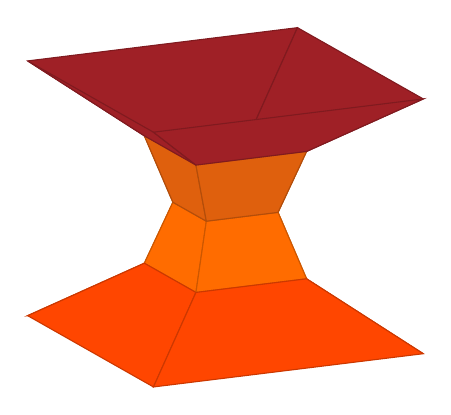
\begin{tikzpicture}
                    \begin{axis}[
                        view={110}{20},
                        samples=\samplescalar,
                        samples y=\samplescalar,
                        domain=0:2*pi,
                        y domain=-2:2,
                        scale = 1,
                        axis lines=none,
                        colormap={orangered}{
                            rgb(0cm)=(1,0.2,0);
                            rgb(1cm)=(1,0.5,0);
                            rgb(2cm)=(0.5,0,0.2);
                        },
                    ]
                    
                    % katenoida
                    \addplot3[
                        surf,
                        z buffer=sort,
                    ]
                    (
                        {cosh(y)*cos(deg(x))},
                        {cosh(y)*sin(deg(x))},
                        {y}
                    );
                    
                    \end{axis}
                \end{tikzpicture}
            
                \caption{Katenoida}
            \end{figure}

        \end{column}

        \begin{column}{0.5\textwidth}
            \begin{definicija}
                Minimalna ploskev v $\mathbb{R}^3$ je taka, ki \textcolor{red1}{lokalno minimizira ploščino} med vsemi bližnjimi ploskvami z istim robom.
            \end{definicija}
            Prva poznana minimalna ploskev. 

            \vspace{0.8em}

            Leta 1744 je Euler dokazal, da je ketenoida minimalna ploskev. Je edina netrivialna \textcolor{red1}{rotacijska minimalna ploskev} v $\mathbb{R}^3$. 
            
            \vspace{0.8em}

            Dobimo jo z rotacijo grafa hiperboličnega kosinusa (t.~i.~“verižnice”) okoli izbrane osi v $\mathbb{R}^3$. Torej
            \begin{gather*}
                x^2+y^2=\cosh^2{z} \\
                (\varphi, z) \mapsto(\cos \varphi \cdot \cosh z, \sin \varphi \cdot \cosh z, z).
            \end{gather*}

        \end{column}
    \end{columns}

\end{frame}

\begin{frame}
    \frametitle{J.~L.~Lagrange 1760 - grafi z minimalno ploščino}

    Naj bo $D$ omejena podmnožica ravnine $\mathbb{R}^2$ z odsekoma $\mathscr{C}^1$ robom $b D$. Naj bo funkcija $f: \overline{D} \rightarrow \mathbb{R}$ razreda $\mathscr{C}^2$ definirana na zaprtju $\overline{D}$. Njen graf je množica točk
    \begin{equation*}
        \mathcal{G}_f=\left\{(x, y, z) \in \mathbb{R}^3 \mid(x, y) \in \overline{D}, z=f(x, y)\right\}    
    \end{equation*}
    in ima površino enako
    \begin{equation*}
        \operatorname{Area}(f)=\iint_{D} \sqrt{1+f_x^2+f_y^2} \, \mathrm{d} x \mathrm{d} y=\iint_{D} \sqrt{1+|\nabla f|^2} \, \mathrm{d} x \mathrm{d} y.    
    \end{equation*}
    Hočemo najti funkcije $f$, ki bodo imele najmanjšo ploščino med vsemi bližnjimi grafi nad $\overline{D}$ z enakimi robnimi vrednostmi.

    \vspace{0.8em}

    Izberemo $\mathscr{C}^1$ funkcijo $h: \overline{D} \rightarrow \mathbb{R}$, za katero velja $h(b D) \equiv 0$. Za $s \in \mathbb{R}$ si ogledamo naslednjo funkcijo:
    \begin{equation*}
        s \longmapsto \operatorname{Area}(f+s h) \in \mathbb{R}_+ .    
    \end{equation*}
    Funkcija $f$ bo stacionarna točka \textcolor{red1}{ploščinskega funkcionala} natanko tedaj, ko bo pri $s=0$ za vse zgoraj opisane deformacije $h$ veljalo
    \begin{equation*}
        \left.\frac{\mathrm{d}}{\mathrm{d} s}\right|_{s=0} \operatorname{Area}(f+s h)=0.
    \end{equation*}
    
\end{frame}

\begin{frame}
    \frametitle{J.~L.~Lagrange 1760 - grafi z minimalno ploščino}

    To lahko razpišemo na
    \begin{align*}
        \left.\frac{\mathrm{d}}{\mathrm{d} s}\right|_{s=0} \operatorname{Area}(f+s h) & =\left.\iint_{D} \frac{\mathrm{d}}{\mathrm{d} s}\right|_{s=0} \sqrt{1+\left(f_x+s h_x\right)^2+\left(f_y+s h_y\right)^2} \, \mathrm{d} x \mathrm{d} y \\
        & =\iint_{D} \frac{f_x h_x+f_y h_y}{\sqrt{1+f_x^2+f_y^2}} \, \mathrm{d} x \mathrm{d} y \\
        & =\iint_{D} \frac{\nabla f \cdot \nabla h}{\sqrt{1+|\nabla f|^2}} \, \mathrm{d} x \mathrm{d} y
    \end{align*}
    Ker poznamo robne vrednosti deformacije $h$ in funkcije $f$ je na tem koraku smiselno uporabiti Gaussov izrek, ki bo zgornji integral po območju povezal integralom po robu tega območja. 

    \vspace{0.8em}

    Če upoštevamo, da za funkcijo $h$ in vektorsko polje $\mathbf{F}$ velja $\operatorname{div}(h \mathbf{F})=\nabla h \cdot \mathbf{F}+h \cdot \operatorname{div}(\mathbf{F})$ dobimo t.~i.~prvo Greenovo identiteto
    \begin{equation*}
        \iint_{D} \nabla h \cdot \mathbf{F} \, \mathrm{d} x \mathrm{d} y=\oint_{b D} h \mathbf{F} \, \mathbf{n} \cdot \mathrm{d} s-\iint_{D} h \cdot \operatorname{div}(\mathbf{F}) \, \mathrm{d} x \mathrm{d} y,
    \end{equation*}
    kjer je $\mathbf{n}$ normala na rob območja. V našem primeru izberemo $\mathbf{F}=\frac{\nabla f}{\sqrt{1+|\nabla f|^2}}$.

\end{frame}

\begin{frame}
    \frametitle{J.~L.~Lagrange 1760 - enačba za minimalne grafe}

    Torej
    \begin{align*}
        \left.\frac{\mathrm{d}}{\mathrm{d} s}\right|_{s=0} \operatorname{Area}(f+s h) & =\iint_{D} \nabla h \cdot \frac{\nabla f}{\sqrt{1+|\nabla f|^2}} \, \mathrm{d} x \mathrm{d} y \\
        & =-\iint_{D}h \cdot \operatorname{div}\left(\frac{\nabla f}{\sqrt{1+|\nabla f|^2}}\right) \, \mathrm{d} x \mathrm{d} y,
    \end{align*}
    Zaradi zveznosti $h$, je izraz enak $0$ za vse izbore $h$ natanko takrat, ko je integrand poleg $h$ identično enak $0$ na $D$. To lahko zapišemo v naslednji obliki
    \begin{equation*}
        \frac{\partial}{\partial x} \frac{f_x}{\sqrt{1+|\nabla f|^2}}+\frac{\partial}{\partial y} \frac{f_y}{\sqrt{1+|\nabla f|^2}}=\frac{\left(1+f_y^2\right) f_{x x}-2 f_x f_y f_{x y}+\left(1+f_x^2\right) f_{y y}}{\left(1+|\nabla f|^2\right)^{3 / 2}}=0 , 
    \end{equation*}
    kar je pa dalje ekvivalentno
    \begin{equation*}
        \mathscr{G}(f)=\left(1+f_y^2\right) f_{x x}-2 f_x f_y f_{x y}+\left(1+f_x^2\right) f_{y y}=0 .
    \end{equation*}
    To je \textcolor{red1}{Euler-Lagrangeova enačba} za ploščinski funkcional. Je eliptična PDE drugega reda, ki jo poznamo pod imenom \textcolor{red1}{enačba za minimalne grafe}.
    
    \vspace{0.8em}
    
    Na tej točki se naravno vprašamo, ali rešitev enačbe za minimalne grafe z zvezno določenimi robnimi vrednostmi na $bD$ sploh obstaja in ali je enolična. Ta Dirichletov problem za enačbo minimalnega grafa je leta 1930 razrešil T.~Radó za omejena konveksna območja $D \subset \mathbb{R}^2$. Rešitev je enolična in absolutno minimizira ploščino med \emph{vsemi} ploskvami s takim robom.

\end{frame}

\begin{frame}
    \frametitle{Ukrivljenost krivulj in ploskev}

    Enačbo za minimalne grafe bi si radi interpretirali na bolj geometrijski način. Pred tem si moramo najprej ogledati koncepta glavnih ukrivljenosti in povprečne ukrivljenosti ploskve v Evklidskem prostoru $\mathbb{R}^n$.

    \begin{aksiom}
        Ukrivljenost krivulje ali ploskve je invariantna za afine linearne preslikave $\mathbb{R}^n \rightarrow \mathbb{R}^n$ oblike $x \mapsto A x+b$, kjer je $b \in \mathbb{R}^n$ in $A \in O_n(\mathbb{R})$ iz ortogonalne grupe na $\mathbb{R}^n$. Takim preslikavam pravimo \textcolor{red1}{toge}.
    \end{aksiom}
    Toge preslikave so ravno izometrije Evklidske metrike na $\mathbb{R}^n$. 

    \vspace{0.8em}

    Enostavna posledica izreka o implicitni funkciji je ta, da lahko vsako gladko krivuljo $C$ okoli točke $p \in C$ predstavimo kot graf nad njeno tangento $T_p C$. Analogna trditev drži za ploskve. 
    
    \vspace{0.8em}

    Najprej si bomo ogledali ukrivljenost gladke krivulje v ravnini, torej $C \subset \mathbb{R}^2$. V tem primeru torej lahko poljubno točko na krivulji $p \in C$, s togim premikom premaknemo v koordinatno izhodišče $(0,0)$, njeno tangento $T_p C$ pa na $x$ os. Torej, lokalno gledano je krivulja $C$ v okolici točke $(0,0)$ graf gladke funkcije $y=f(x)$, definirane na intervalu okoli $0 \in \mathbb{R}$. Očitno velja $f(0)=f^{\prime}(0)=0$. Taylorjev razvoj $f$ pri $0$ se potem glasi
    \begin{equation*}
        y=f(x)=\frac{1}{2} f^{\prime \prime}(0) x^2+o\left(x^2\right),
    \end{equation*}
    kjer je $h(x)=o\left(x^2\right) \stackrel{\text { def }}{\iff} \lim _{x \rightarrow 0} \frac{h(x)}{x^2}=0$.

\end{frame}

\begin{frame}
    \frametitle{Ukrivljenost krivulj}

    Najdimo zdaj radij krožnice, ki se bo najbolje prilegala razvoju te funkcije v točki $(0,0)$. Očitno je, da ima ta krožnica središče na $y$ osi in se dotika grafa v točki $(0,0)$, torej je oblike
    \begin{equation*}
        x^2+(y-r)^2=r^2
    \end{equation*}
    za nek $r \in \mathbb{R} \setminus \{0\}$, razen v primeru, ko je $f^{\prime \prime}(0)=0$, kadar pa dobimo $r=\infty$. Če to enačbo razrešimo na $y$ v okolici $(0,0)$ dobimo 
    \begin{equation*}
        y=r-\sqrt{r^2-x^2}=r-r \sqrt{1-\frac{x^2}{r^2}}=r-r\left(1-\frac{x^2}{2 r^2}+o\left(x^2\right)\right)=\frac{1}{2 r} x^2+o\left(x^2\right).
    \end{equation*}
    Primerjava dobljene enačbe z enačbo razvojem $f$ nam pokaže, da je za $f^{\prime \prime}(0)\neq0$ 
    \begin{equation*}
        r=1 / f^{\prime \prime}(0) \in \mathbb{R} \setminus \{0\}
    \end{equation*}
    enolično določa radij, pri katerim se krožnica najbolje ujema s krivuljo $C$ v točki $(0,0)$. Taki krožnici pravimo \textcolor{red1}{pritisnjena krožnica}, recipročni vrednosti radija 
    \begin{equation*}
        \kappa=f^{\prime \prime}(0)=1 / r
    \end{equation*}
    pa \textcolor{red1}{predznačena ukrivljenost} krivulje v $(0,0)$. Njeno absolutno vrednost $|\kappa|=\left|f^{\prime \prime}(0)\right| \geq 0$ imenujemo \textcolor{red1}{ukrivljenost}, $|r|=1 /|\kappa|=1 /\left|f^{\prime \prime}(0)\right|$ pa \textcolor{red1}{krivinski radij}. 

\end{frame}

\begin{frame}
    \frametitle{Ukrivljenost ploskev}

    Naj bo $S \subset \mathbb{R}^3$ gladka ploskev. Na ploskvi fiksiramo točko $p \in S$. S togo preslikavo lahko premaknemo $p$ v $(0,0,0)$ in $T_p S$ v $\mathbb{R}^2 \times\{0\}$. Potem lahko, $S$ okoli koorinatnega izhodišča izrazimo kot graf oblike 
    \begin{equation*}
        z=f(x, y)=\frac{1}{2}\left(f_{x x}(0) x^2+2 f_{x y}(0,0) x y+f_{y y}(0) y^2\right)+o\left(x^2+y^2\right). 
    \end{equation*}
    Označimo z $A$ Hessjevo matriko funkcije $f$ v točki $(0,0)$:
    \begin{equation*}
        A=\begin{bmatrix}
            f_{x x}(0,0) & f_{x y}(0,0) \\
            f_{x y}(0,0) & f_{y y}(0,0)
        \end{bmatrix} .
    \end{equation*}
    Izberemo si zdaj enotski vektor $v=\left(v_1, v_2\right)$ v $(x,y)$ ravnini. S $\Sigma_v$ označimo ravnino skozi koordinatno izhodišče, ki jo razpenjata vektor $v$ in koordinatna os $z$. Presečišče $C_v:=S \cap \Sigma_v$ je krivulja na $S$ parametrizirana z
    \begin{equation*}
        z=f\left(v_1 t, v_2 t\right)=\frac{1}{2}(A v \cdot v) t^2+o\left(t^2\right)
    \end{equation*}
    za $t \in \mathbb{R}$ blizu $0$. Iz prejšnje drsnice o ukrivljenosti krivulj in dobljene formule vemo, da je 
    \begin{equation*}
        \kappa_v=A v \cdot v=f_{x x}(0) v_1^2+2 f_{x y}(0,0) v_1 v_2+f_{y y}(0) v_2^2
    \end{equation*}
    predznačena ukrivljenost krivulje $C_v$ v točki $(0,0)$.
    
\end{frame}

\begin{frame}
    \frametitle{Ukrivljenost ploskev}

    \begin{figure}
        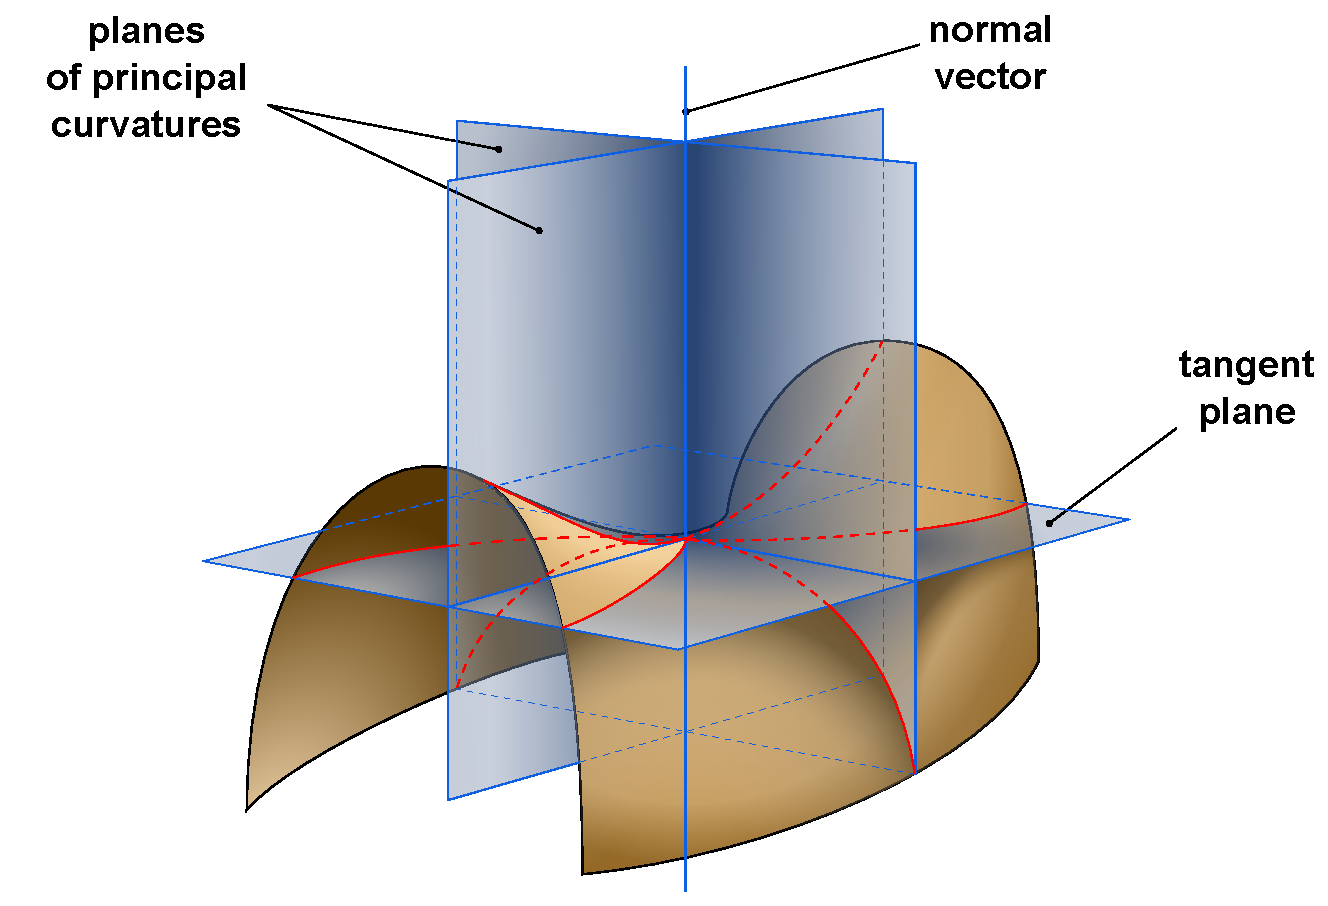
\includegraphics[width=20em]{../Slike/Minimal_surface_curvature_planes.pdf}
    \end{figure}

    Na enotski krožnici $|v|^2=v_1^2+v_2^2=1$ kvadratna forma $v \mapsto A v \cdot v$ doseže svoj maksimum $\kappa_1$ in minimum $\kappa_2$; ti dve vrednosti imenujemo \textcolor{red1}{glavni ukrivljenosti} ploskve $S$ v točki $0$. Ker je matrika $A$ simetrična sta $\kappa_1$ in $\kappa_2$ njeni lastni vrednosti. Vrednosti 
    \begin{equation*}
        H=\frac{1}{2}(\kappa_1+\kappa_2)=\operatorname{sl} A, \quad K=\kappa_1 \kappa_2=\operatorname{det} A
    \end{equation*}
    imenujemo \textcolor{red1}{povprečna ukrivljenost} in \textcolor{red1}{Gaussova ukrivljenost} ploskve $S$ v točki $0$. 

    \vspace{0.8em}

    Sled matrike $A$ je enaka $\bigtriangleup f(0,0)=f_{x x}(0,0)+f_{y y}(0,0)$. Po drugi strani, pa je sled matrike enaka vsoti njenih lastnih vrednosti. To implicira 
    \begin{equation*}
        \bigtriangleup f(0,0)=\kappa_1+\kappa_2=2H.
    \end{equation*}

\end{frame}

\begin{frame}
    \frametitle{Geometrijska interpretacija enačbe za minimalne grafe}

    Naslednjo trditev je leta 1776 dokazal Meusnier in s tem karakteriziral minimalne grafe s srednjo ukrivljenostjo. 
    \begin{izrek}
        Funkcija $f: D \rightarrow \mathbb{R}$ razreda $\mathscr{C}^2$, definirana na domeni $D \subset \mathbb{R}^2$ reši enačbo za minimalne grafe 
        \begin{equation*}
            \mathscr{G}(f):=\left(1+f_y^2\right) f_{x x}-2 f_x f_y f_{x y}+\left(1+f_x^2\right) f_{y y}=0 
        \end{equation*}
        natanko tedaj, ko ima njen graf $S=\mathcal{G}_f$ v vsaki točki  ničelno srednjo ukrivljenost. 
    \end{izrek}

    \emph{Dokaz:}

    Izberimo točko $p_0\in D$. Evklidske koordinate, ki ohranijo $z$ smer izberemo tako, da velja $p_0=(0,0)$, $f(0,0)=0$ in 
    \begin{equation*}
        f(x, y)=a x+O\left(x^2+y^2\right), \quad \text{za }  a \geq 0.    
    \end{equation*}
    
    Ekvivalenco iz trditve je zato dovolj dokazati v točki $(0,0)$. Izberimo si naslednjo ortonormirano bazo $\mathbb{R}^3$:
    \begin{equation*}
        \mathbf{v}_1=\frac{1}{\sqrt{1+a^2}}(1,0, a), \quad \mathbf{v}_2=(0,1,0), \quad \mathbf{v}_3=\frac{1}{\sqrt{1+a^2}}(-a, 0,1).
    \end{equation*}
    Vidimo, da $\mathbf{v}_1$ in $\mathbf{v}_2$ razpenjata tangentno $T_0 S$ ravnino v $(0,0)$, $\mathbf{v}_3$ pa je normala na $T_0S$. Označimo z $(u, v, w)$ Evklidske koordinate, ki so vezane na to bazo. 
     
\end{frame}

\begin{frame}
    \frametitle{Dokaz Meusnierjevega izreka}

    Torej se prvotne koordinate izrazijo kot 
    \begin{equation*}
        (x, y, z)=u \mathbf{v}_1+v \mathbf{v}_2+w \mathbf{v}_3.
    \end{equation*}
    V koordinatah $(u,v,w)$ je ploskev $S$ na okolici koordinatnega izhodišča podana kot graf oblike
    \begin{equation*}
        w=g(u, v), \quad g(0,0)=0, \quad \mathrm{d} g(0,0)=0.
    \end{equation*}
    Vemo, da je srednja ukrivljenost $S$ v točki $(0,0)$ enaka $2H=\bigtriangleup g(0,0)$. Za dokončanje dokaza bomo $g$ prevedli na $f$ in izrazili $\mathscr{G}(f)(0,0)$ z $\bigtriangleup g(0,0)$. 
    
    \vspace{0.8em}
    V koordinatah $(x, y, z)$ je ploskev $S$ parametrizirana kot 
    \begin{equation*}
        x=\frac{1}{\sqrt{1+a^2}}(u-a g(u, v)), \quad y=v, \quad z=\frac{1}{\sqrt{1+a^2}}(a u+g(u, v)) .
    \end{equation*}
    Ker je $S$ prav tako podana z $z=f(x, y)$ dobimo izraz
    \begin{equation*}
        a u+g(u, v)=\sqrt{1+a^2} \cdot f\left(\frac{u-a g(u, v)}{\sqrt{1+a^2}}, v\right) .
    \end{equation*}
    Ta izraz zdaj dvakrat odvajamo po $u$ in po $v$: 
    \begin{align*}
        g_{u u} & =f_{x x}\left(1-a g_u\right)^2 / \sqrt{1+a^2}+f_x\left(-a g_{u u}\right) \\
        g_{v v} & =f_{x x}\left(-a g_v\right)^2 / \sqrt{1+a^2}+f_x\left(-a g_{v v}\right)+f_{x y}\left(-2 a g_v\right)+f_{y y} \sqrt{1+a^2} .
    \end{align*}
    
\end{frame}

\begin{frame}
    \frametitle{Dokaz Meusnierjevega izreka}

    Če ovrednotimo druge parcialne odvode pri $(u, v)=(0,0)$, kar se ujema z $(x, y)=(0,0)$ in upoštevamo $f_x(0,0)=a, f_y(0,0)=0, g_u(0,0)=g_v(0,0)=0$ dobimo 
    \begin{align*}
        g_{u u}(0,0) & =f_{x x}(0,0) / \sqrt{1+a^2}-a^2 g_{u u}(0,0) \\
        g_{v v}(0,0) & =-a^2 g_{v v}(0,0)+f_{y y}(0,0) \sqrt{1+a^2}
    \end{align*}
    in tako 
    \begin{equation*}
        f_{x x}(0,0)={\sqrt{1+a^2}}^3 g_{u u}(0,0), \quad f_{y y}(0,0)=\sqrt{1+a^2} g_{v v}(0,0)
    \end{equation*}
    Tako pri $(0,0)$ dobimo
    \begin{align*}
        \mathscr{G}(f) & =\left(1+f_y^2\right) f_{x x}-2 f_x f_y f_{x y}+\left(1+f_x^2\right) f_{y y} \\
        & ={\sqrt{1+a^2}}^3 g_{u u}+\left(1+a^2\right) \sqrt{1+a^2} g_{v v} \\
        & ={\sqrt{1+a^2}}^3 \bigtriangleup g .
    \end{align*}
    To pokaže, da je $\mathscr{G}(f)(0,0)=0$ natanko tedaj, ko je $\bigtriangleup g(0,0)=2H=0$. \hfill $\square$

    \begin{definicija}
        Gladka ploskev v $\mathbb{R}^3$ je \textcolor{red1}{minimalna}, če je njena povprečna ukrivljenost v vsaki točki ničelna, t.~j.~$\frac{1}{2}(\kappa_1+\kappa_2)=0$.
    \end{definicija}
\end{frame}

\begin{frame}
    \frametitle{J.~B.~Meusnier - 1776 - Helikoid}
    \begin{columns}
        \begin{column}{0.5\textwidth}
            \centering
            \begin{figure}[H]
                \centering
                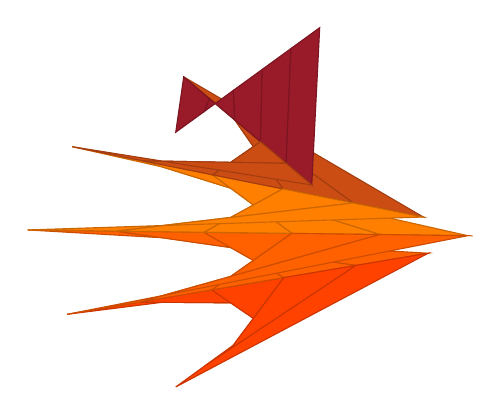
\begin{tikzpicture}
                    \begin{axis}[
                        view={110}{20},
                        samples=\samplescalar*1.2,
                        samples y=\samplescalar*1.2,
                        domain=-2:2,
                        y domain=0:4*pi,
                        scale = 1,
                        axis lines=none,
                        colormap={orangered}{
                            rgb(0cm)=(1,0.2,0);
                            rgb(1cm)=(1,0.5,0);
                            rgb(2cm)=(0.5,0,0.2);
                        },
                    ]
                    
                    % helikoid
                    \addplot3[
                        surf,
                        z buffer=sort,
                    ]
                    (
                        {x * cos(deg(y))}, 
                        {x * sin(deg(y))}, 
                        {y} 
                    );
                    
                    \end{axis}
                \end{tikzpicture}
            
                \caption{Helikoid}
            \end{figure}
        \end{column}

        \begin{column}{0.5\textwidth}
            Meusnier je leta 1776 dokazal, da je helikoid minimalna ploskev. 
            
            \vspace{0.8em}

            Dobimo ga tako, da premico v $\mathbb{R}^2$ vrtimo in jo hkrati dvigujemo v smeri osi vrtenja. V kartezičnih koordinatah je podan kot
            \begin{align*}
                & x=\rho \cos (\theta), \\
                & y=\rho \sin (\theta), \\
                & z=\theta,
            \end{align*}
            za $\rho$ in $\theta$ od $-\infty$ do $\infty$.

            \vspace{0.8em}
            
            Poleg ravnine je to edina minimalna ploskev, ki jo lahko predstavimo kot unijo premic. Take ploskve imenujemo \textcolor{red1}{premonosne plokve}.
            
        \end{column}
    \end{columns}
\end{frame}

\begin{frame}
    \frametitle{Scherkova ploskev - 1835}

    Heinrich Scherk leta 1835 odkrije 2 novi minimalni ploskvi. Prve nove odkrite minimalne ploskve po helikoidu.

    \vspace{0.8em}

    \begin{columns}
        \begin{column}{0.5\textwidth}
            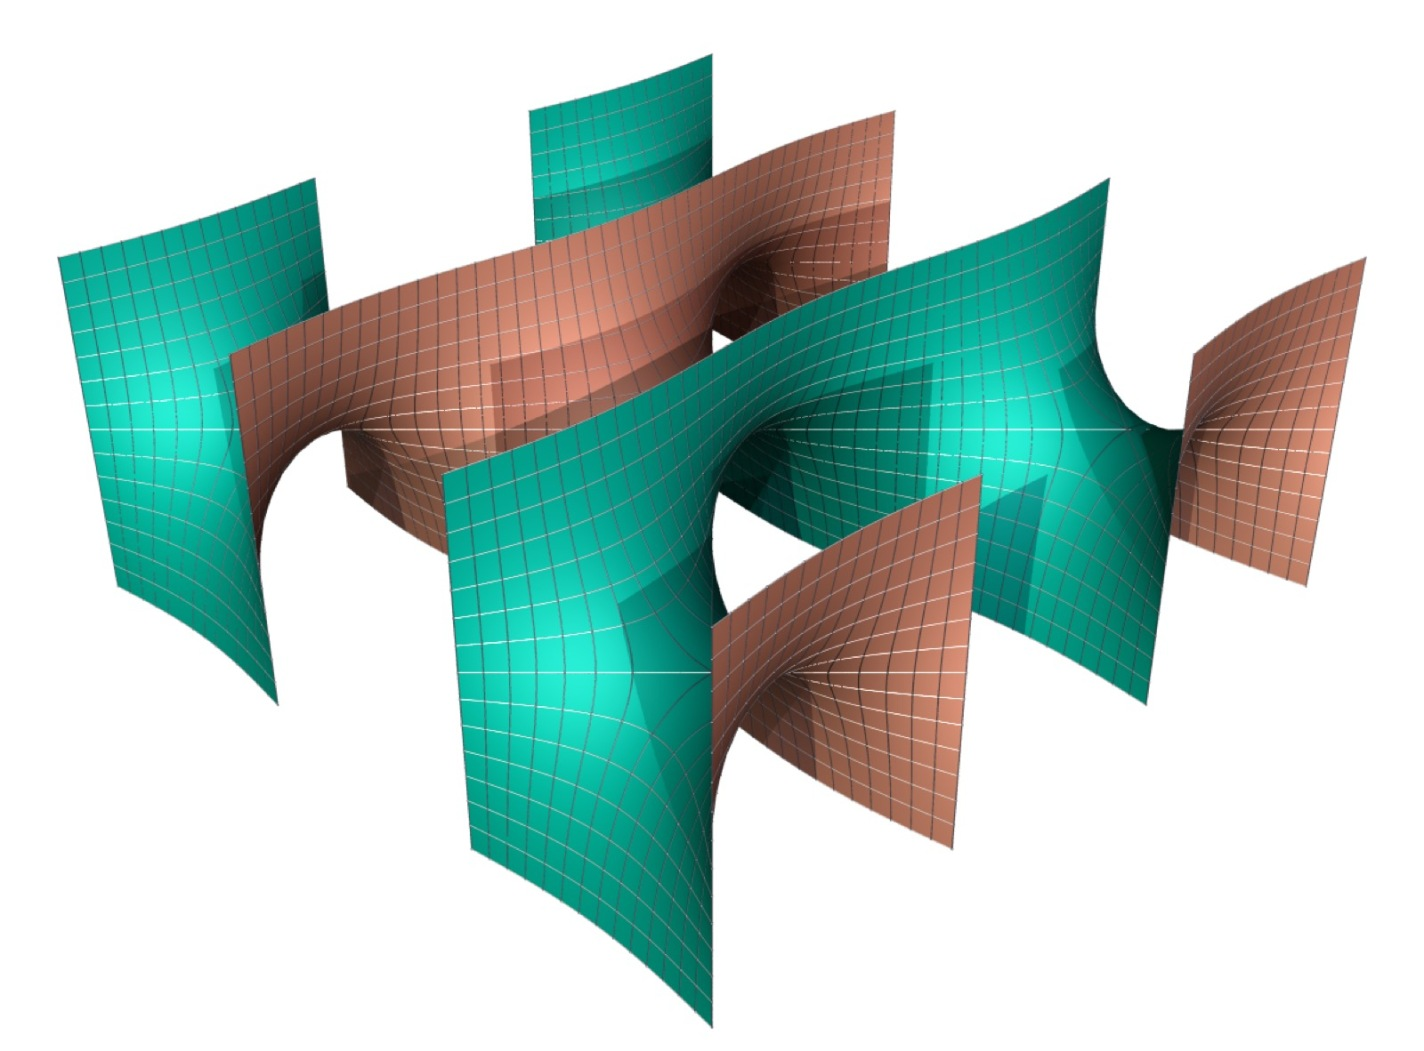
\includegraphics[width=20em]{../Slike/Scherk_Minimal_Surface.jpg}
            %\centering
            %\begin{figure}[H]
            %    \centering
            %    \begin{tikzpicture}
            %        \begin{axis}[
            %            view={60}{30},
            %            samples = \samplescalar/2,
            %            samples y=\samplescalar/2,
            %            domain=-pi/2+0.001:pi/2-0.001, 
            %            zmin=-0.4, zmax=0.4,
            %            clip=false,
            %            scale = 0.28,
            %            axis lines=none,
            %            colormap={orangered}{
            %                rgb(0cm)=(1,0.2,0);
            %                rgb(1cm)=(1,0.5,0);
            %                rgb(2cm)=(0.5,0,0.2);
            %            },
            %            ]
%
            %            % scherkova ploskev
            %            \addplot3[
            %                surf, 
            %                shader=faceted interp,
            %            ] 
            %            (
            %                {x}, 
            %                {y}, 
            %                {log10(cos(deg(x))/cos(deg(y)))} 
            %            );
            %        \end{axis}
            %    \end{tikzpicture}
            %    \caption{Sherkova ploskev}
            %\end{figure}
        \end{column}

        \begin{column}{0.5\textwidth}
            Prva Scherkova ploskev je invariantna pod dvema ortogonalnima translacijama, torej je dvojno preiodična. Njena glavna veja je graf nad kvadratom $P=\left(-\frac{\pi}{2}, +\frac{\pi}{2}\right)^2$, podana kot
            \begin{equation*}
                z = \ln{\cos{y}} - \ln{\cos{x}}
            \end{equation*}
            Ta Scherkova ploskev ima največjo Gaussovo ukrivljenost v $0\in \mathbb{R}^3$ izmed vseh minimalnih grafov, ki ležijo nad kvadratom $P$, in sicer $-1$. 

            \vspace{0.8em}

            %\begin{figure}[H]
            %    \center
            %    \begin{tikzpicture}[scale=0.15] 
            %        \pgfmathsetmacro{\twopi}{2*pi}
            %        \pgfmathsetmacro{\halfpi}{pi/2}
            %        
            %        % Sivi kvadrati
            %        \foreach \n in {-1,0,1} {
            %          \foreach \m in {-1,0,1} {
            %            \pgfmathsetmacro\xmin{-\halfpi + \n*\twopi}
            %            \pgfmathsetmacro\xmax{\halfpi + \n*\twopi}
            %            \pgfmathsetmacro\ymin{-\halfpi + \m*\twopi}
            %            \pgfmathsetmacro\ymax{\halfpi + \m*\twopi}
            %            \fill[lightgray] (\xmin,\ymin) rectangle (\xmax,\ymax);
            %          }
            %        }
            %        
            %        \foreach \n in {-0.5,0.5} {
            %          \foreach \m in {-0.5,0.5} {
            %            \pgfmathsetmacro\xmin{-\halfpi + \n*\twopi}
            %            \pgfmathsetmacro\xmax{\halfpi + \n*\twopi}
            %            \pgfmathsetmacro\ymin{-\halfpi + \m*\twopi}
            %            \pgfmathsetmacro\ymax{\halfpi + \m*\twopi}
            %            \fill[lightgray] (\xmin,\ymin) rectangle (\xmax,\ymax);
            %          }
            %        }
            %        
            %        % Crtkane crte
            %        \foreach \n in {-1,0,1} {
            %          \pgfmathsetmacro\xleft{-\halfpi + \n*pi}
            %          \pgfmathsetmacro\xright{\halfpi + \n*pi}
            %        
            %          % Vertikalne
            %          \draw[dashed, gray] (\xleft,-10) -- (\xleft,10);
            %          \draw[dashed, gray] (\xright,-10) -- (\xright,10);
            %        
            %          % Horizontalne 
            %          \pgfmathsetmacro\ybot{-\halfpi + \n*pi}
            %          \pgfmathsetmacro\ytop{\halfpi + \n*pi}
            %          \draw[dashed, gray] (-10,\ybot) -- (10,\ybot);
            %          \draw[dashed, gray] (-10,\ytop) -- (10,\ytop);
            %        }
            %        
            %        % Oznake
            %        %\foreach \x/\xlabel in {-4.712/{\small $-\frac{3\pi}{2}$}, -1.571/{\small $-\frac{\pi}{2}$}, 1.571/{\small $\frac{\pi}{2}$}, 4.712/{\small $\frac{3\pi}{2}$}} {
            %        %  \draw[thick] (\x,0.2) -- (\x,-0.2);
            %        %  \node[below] at (\x,-0.05) {\xlabel};
            %        %}
            %        %    
            %        %\foreach \y/\ylabel in {-4.712/{\small $-\frac{3\pi}{2}$}, -1.571/{\small $-\frac{\pi}{2}$}, 1.571/{\small $\frac{\pi}{2}$}, 4.712/{\small $\frac{3\pi}{2}$}} {
            %        %  \draw[thick] (0.2,\y) -- (-0.2,\y);
            %        %  \node[left] at (-0.05,\y) {\ylabel};
            %        %}
            %        
            %        % Osi
            %        \draw[->, thick] (-10, 0) -- (10, 0) node[right] {$x$};
            %        \draw[->, thick] (0, -10) -- (0, 10) node[above] {$y$};
            %        
            %    \end{tikzpicture}
            %    \caption{Definicijsko območje Sherkove ploskve}
            %\end{figure}
            
        \end{column}
    \end{columns}

    \textcolor{red1}{Torej, če hočemo, da graf minimalne ploskve obstaja nad določeno domeno, potem ne mora biti poljubno ukrivljen.} 
    
    \vspace{0.8em}

    Minimalen graf v $\mathbb{R}^3$ nad celotno ravnino je ravnina. 

\end{frame}

\begin{frame}
    \frametitle{Riemannovi minimalni primeri - 1867}

    \begin{columns}
        \begin{column}{0.4\textwidth}
            \centering
            \begin{figure}
                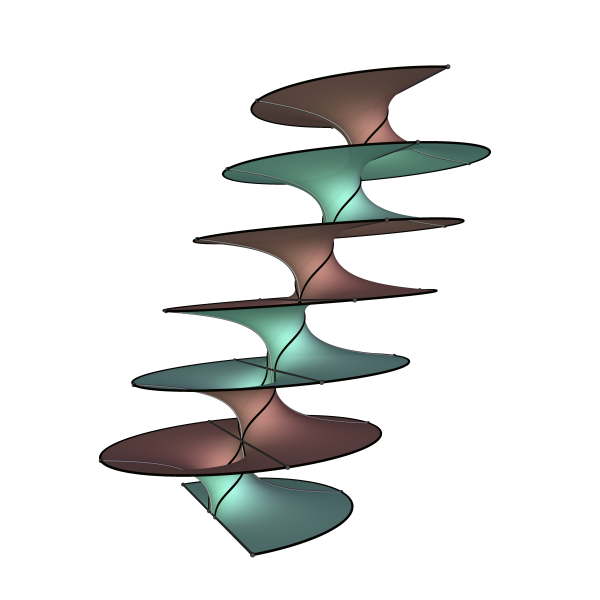
\includegraphics[width=16em]{../Slike/Riemann_Minimal_Example.png}
                \caption{Eden Riemannovih minimalnih primerov}
            \end{figure}
        \end{column}

        \begin{column}{0.6\textwidth}
            Proti koncu svojega življenja je Bernhard Riemann odkril družino enoparametričnih minimalnih ploskev $R_\lambda$ za $\lambda \in (0, \infty)$. Parametrizirane so s periodičnimi ravninskimi domenami in so \textcolor{red1}{pravilno vložene} kot minimalne ploskve v $\mathbb{R}^3$. Vsaka horizontalna ravnina se s ploskvijo seka v premici ali pa krožnici. Ko pošljemo $\lambda \rightarrow 0$ te ploskve konvergirajo h katenoidi, če pa pošlejmo $\lambda \rightarrow \infty$ konvergirajo h helikoidu. 

            \vspace{0.8em}

            \textcolor{red1}{Topološka definicija pravline vložitve:} preslikava je pravilna vložitev, če je vložitev in če dodatno velja, da so praslike kompaktov kompakti.
            
            \vspace{0.8em}

            Meeks, Pérez, Ros so 2015 dokazali, da so helikoidi, katenoidi in Riemannovi minimalni prmeri edine ravninske domene, ki jih lahko pravlino vložimo kot minimalne ploskve v $\mathbb{R}^3$. Imerzij seveda obstaja veliko več. 
        \end{column}
    \end{columns}
    
\end{frame}

\begin{frame}
    \frametitle{Hennebergova ploskev - 1875}

    \begin{columns}
        \begin{column}{0.5\textwidth}
            \centering
            \begin{figure}[H]
                \centering
                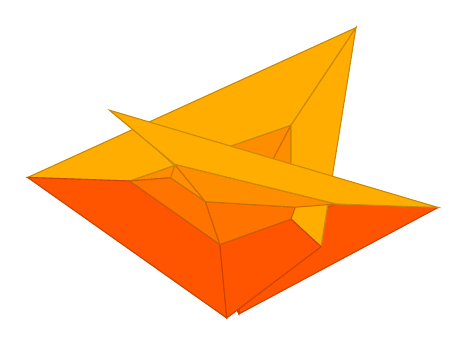
\begin{tikzpicture}
                    \begin{axis}[
                        view={130}{20},
                        samples=\samplescalar,
                        samples y=\samplescalar,
                        domain=0:2*pi,
                        y domain=-1.5:1.5,
                        axis lines=none,
                        colormap/redyellow,
                        z buffer=sort,
                    ]
                    \addplot3[
                        surf,
                    ]
                    (
                        {cosh(y)*sin(deg(x)) - sinh(y)*cos(deg(2*x))},
                        {cosh(y)*cos(deg(x)) + sinh(y)*sin(deg(2*x))},
                        {2*sinh(y)*sin(deg(x))}
                    );
                    \end{axis}
                    
                \end{tikzpicture}
                \caption{Hennebergova ploskev}
            \end{figure}
        \end{column}

        \begin{column}{0.5\textwidth}
            \textcolor{red1}{Neorientabilna minimalna ploskev}. 
            
            Ni vložitev. Do 1981 edina poznana neorientabilna minimlana ploskev. 

            \vspace{0.8em}

            Meeks leta 1981 odkrije pravilno imerzijo Möbiusovega traku v $\mathbb{R}^3$. 2017 je odkrita tudi pravilna vložitev Möbisuovega traku v $\mathbb{R}^4$.
        \end{column}
    \end{columns}
    
\end{frame}

\begin{frame}
    \frametitle{Analitičen opis konformnih minimalnih ploskev}

    Izberimo koordinate $(u,v)$ na $\mathbb{R}^2$. Naj bo $D \subset \mathbb{R}^2$ omejeno območje z gladkim robom. 
    \begin{definicija}[Imerzija]
        Preslikava $F: D \rightarrow \mathbb{R}^n$ $(n \geq 2)$ razreda $\mathscr{C}^1$ je \textcolor{red1}{imerzija}, če sta parcialna odvoda $F_u=\partial F / \partial u$ in $F_v=\partial F / \partial v$ linearno neodvisna v vsaki točki $D$. 
    \end{definicija}
    Naj bo $F: \overline{D} \rightarrow \mathbb{R}^n$ gladka imerzija. Predpostavimo, da lahko koordinate $(u,v)$ izberemo tako, da je $F$ \textcolor{red1}{konformna preslikava}. To pomeni, da bo zanjo veljalo
    \begin{equation*}
        \left|F_u\right|=\left|F_v\right| , \quad F_u \cdot F_v=0.
    \end{equation*}
    Ta predpostavka sledi iz obstoja izotermalnih koordinat, kar bomo utemeljili kasneje. Poglejmo si spet \textcolor{red1}{ploščinski funkcional}, ki ga lahko zapišemo kot
    \begin{equation*}
        \operatorname{Area}(F)=\iint_D\left|F_u \times F_v\right| \, \mathrm{d} u \mathrm{d} v=\iint_D \sqrt{\left|F_u\right|^2\left|F_v\right|^2-\left|F_u \cdot F_v\right|^2} \, \mathrm{d} u \mathrm{d} v
    \end{equation*}
    in \textcolor{red1}{Dirichletov energetski funkcional}
    \begin{equation*}
        \mathscr{D}(F)=\frac{1}{2} \iint_D|\nabla F|^2 \, \mathrm{d} u \mathrm{d} v=\frac{1}{2} \iint_D\left(\left|F_u\right|^2+\left|F_v\right|^2\right) \, \mathrm{d} u \mathrm{d} v
    \end{equation*}
    Iz neenakosti 
    \begin{equation*}
        |x|^2|y|^2-|x \cdot y|^2 \leq|x|^2|y|^2 \leq \frac{1}{4}\left(|x|^2+|y|^2\right)^2, \quad \text{za }x, y \in \mathbb{R}^n         
    \end{equation*}
    vidimo, da velja $\operatorname{Area}(F) \leq \mathscr{D}(F)$, kjer velja enakost natanko tedaj, ko je $F$ konformna. 
    
\end{frame}

\begin{frame}
    \frametitle{Konformna imerzija je minimalna natanko tedaj, ko je harmonična}

    Torej imata funkcionala $\operatorname{Area}$ in $\mathscr{D}$ iste stacionarne točke na množici konformnih imerzij.

    \vspace{0.8em}

    Izračunajmo prvo variacijo funkcionala $\mathscr{D}$. Če je $h: \overline{D} \rightarrow \mathbb{R}^n$ gladka preslikava, za katero velja $h(bD)\equiv 0$, potem po uporabi prve Greenove identitete v zadnjem enačaju dobimo
    \begin{align*}
        \delta_h \mathscr{D}(F)=\left.\frac{\mathrm{d}}{\mathrm{d} t}\right|_{t=0} \mathscr{D}(F+t h) &=\iint_D\left(F_u \cdot h_u+F_v \cdot h_v\right) \, \mathrm{d} u \mathrm{d} v \\
        &=\iint_D \nabla F \cdot \nabla h \, \mathrm{d} u \mathrm{d} v \\
        &=-\iint_D \operatorname{div}(\nabla F) \cdot h \, \mathrm{d} u \mathrm{d} v.
    \end{align*}
    Ta izraz je enak $0$ za poljuben $h$ natanko tedaj, ko je $\operatorname{div}(\nabla F)= \bigtriangleup X \equiv 0$. S tem smo dokazali naslednji izrek.
    \begin{izrek}
        Konformna imerzija $F: D \rightarrow \mathbb{R}^n$ $(n \geq 3)$ razreda $\mathscr{C}^2$ je stacionarna točka ploščinskega funkcionala natanko tedaj, ko je $F$ harmonična.
    \end{izrek}

\end{frame}

\begin{frame}
    \frametitle{Konformna imerzija je minimalna natanko tedaj, ko je harmonična}

    Imerzija $F: D \rightarrow \mathbb{R}^n$ na $D$ določi Riemannovo metriko $g$, ki ji pogosto pravimo tudi prva fundamentalna forma, podano s formulo
    \begin{equation*}
        g=\left|F_u\right|^2 \mathrm{d} u^2+\left(F_u \cdot F_v\right)(\mathrm{d} u \mathrm{d} v+\mathrm{d} v \mathrm{d} u)+\left|F_v\right|^2 \mathrm{d} v^2 = F^* \mathrm{d}s^2    
    \end{equation*}
    Identiteta $\delta_h \mathscr{D}(F)=-\iint_D \bigtriangleup F \cdot h \, \mathrm{d} u \mathrm{d} v$ pove še več. Količini
    \begin{equation*}
        \frac{2}{\left| \nabla F\right|^2} \bigtriangleup F=\bigtriangleup_g F       
    \end{equation*}
    pravimo intrinzični Laplaceov operator imerzije $F$ glede na Riemannovo metriko $g$ na $D$. Označimo z $\mathrm{d} A=\frac{1}{2}|\nabla F|^2 \, \mathrm{d} u \mathrm{d} v$ diferencial ploščine ploskve. Torej lahko zgornjo identiteto zapišemo kot 
    \begin{align*}
        \delta_h \operatorname{Area}(F)=\left.\frac{\mathrm{d}}{\mathrm{d} s}\right|_{s=0} \operatorname{Area}(F+s h)&=\int_D \nabla \operatorname{Area}(F) \cdot h \, \mathrm{d} A \\
        &=-\int_D \bigtriangleup_g F \cdot h \, \mathrm{d} A.    
    \end{align*}
    To je \textcolor{red1}{formula za prvo variacijo ploščine} imerzije ploskve. Pove nam, da je \textcolor{red1}{vektorsko polje} $\bigtriangleup_g X$ \textcolor{red1}{negativen gradient ploščinskega funkcionala v} $F$.  

\end{frame}

\begin{frame}
    \frametitle{Izotermalne koordinate}

    Naj bo $M$ gladka ploskev in $F: M \rightarrow \mathbb{R}^n$ gladka imerzija, ki na $M$ določi Riemannovo metriko $g = F^* \mathrm{d}s^2$. Za vsako točko $p \in M$ obstaja okolica $U \subset M$ s koordinatami $(\tilde{u}, \tilde{v})$ v katerih Riemannova metrika $g$ dobi enostavnejšo obliko 
    \begin{equation*}
        g=\lambda(u,v)\left(\mathrm{d} \tilde{u}^2+\mathrm{d} \tilde{v}^2\right) \quad \text{za } \lambda(u,v) > 0.
    \end{equation*}
    Vsakim takim koordinatam $(\tilde{u}, \tilde{v})$ pravimo \textcolor{red1}{izotermalne koordinate} za Riemannovo metriko $g$. Naj bo $\widetilde{F}=\widetilde{F}(\tilde{u}, \tilde{v})$ imerzija $U \rightarrow \mathbb{R}^n$, ki jo dobimo iz $F$, če $(u, v)$ izrazimo z $(\tilde{u}, \tilde{v})$. Dobimo 
    \begin{equation*}
        \left|\widetilde{F}_{\tilde{u}}\right|^2=\left|\widetilde{F}_{\tilde{v}}\right|^2=\lambda, \quad \widetilde{F}_{\tilde{u}} \cdot \widetilde{F}_{\tilde{v}}=0,
    \end{equation*}
    kar pomeni, da je $\widetilde{F}: U \rightarrow \mathbb{R}^n$ konformna imerzija. Obstoj izotermalnih koordinat je odkril C.~F.~Gauss za rotacijske ploskve. Dokaz v splošnem je zahteven. 

    \vspace{0.8em}

    Izotermalne koordinate vedno obstajajo, vendar le lokalno. Kaj pa \textcolor{red1}{globalna situacija}? Po tem, kar smo povedali zgoraj vemo, da obstaja odprta povezana okolica $U_i\subset M$ točke $p$, ki jo lahko parametriziramo z gladkim difeomorfizmom $\phi_i^{-1}: V_i\subset \mathbb{R}^2 \rightarrow U_i$, tako da je $F \circ \phi_i^{-1}: V_i \rightarrow \mathbb{R}^n$ konformna vložitev. Če je $\phi_j^{-1}:V_j\subset \mathbb{R}^2 \rightarrow U_j$, $i\neq j$, še ena taka lokalna parametrizacija dela ploskve $U_j\subset M$, kjer velja $U_{ij}=U_i\cap U_j \neq \emptyset$, potem je \textcolor{red1}{prehodna preslikava} $\phi_{ij}=\phi_j \circ \phi_i^{-1}: \phi_i\left(U_{i j}\right) \rightarrow \phi_j\left(U_{i j}\right)$ konformni difeomorfizem med ravninskima domenama. Če $\mathbb{R}^2$ identificiramo s kompleksno ravnino $\mathbb{C}$, vemo, da so konformni difeomorfizmi med pari povezanih odprtih domen v $\mathbb{C}$ ali biholomorfni ali pa antibiholomorfni, glede na to, če ohranijo orientacijo. 
    
\end{frame}

\begin{frame}
    \frametitle{Konformne parametrizacije z Riemannovimi ploskvami}

    Paru $\left(U_i, \phi_i\right)$, kjer je $U_i \subset M$ in $\phi_i$ lokalna parametrizacija pravimo \textcolor{red1}{lokalna karta} na $M$. Zbirki vseh lokalnih kart, ki pokrijejo $M$, t.~j.~$\mathcal{U}=\left\{\left(U_i, \phi_i\right) \mid i \in I\right\}$, kjer je $\left\{U_i\right\}_{i \in I}$ odprto pokritje $M$, pravimo \textcolor{red1}{atlas}. Če so prehodne preslikave $\phi_{ij}$ konfromne atlasu $\mathcal{U}$ pravimo \textcolor{red1}{konformna struktura} na $M$. Ploskev $M$, opremljena z ekvivalenčnim razredom atlasa $\mathcal{U}$, kjer sta dva konformna atlasa ekvivalentna natanko tedaj, ko je njuna unija spet konformen atlas, je \textcolor{red1}{konformna ploskev}. Če je $M$ orientabilna in v konformnem atlasu izberemo za prehodne preslikave $\phi_i$ biholomorfne funkcije, dobimo \textcolor{red1}{Riemannovo ploskev} $(M, \mathcal{U})$. 
    
    \vspace{0.8em}

    Za konformno ploskev $M$ je princip konformne imerzije $M \rightarrow \mathbb{R}^n$ dobro definiran, če nanjo gledamo v lokalnih koordinatah, določenih s konformnim atlasom. Tudi definicija harmonične funkcije je dobra v lokalnih koordinatah.
    \begin{posledica}
        Vsako minimalno ploskev v $\mathbb{R}^n$ lahko parametriziramo s konformno harmonično preslikavo iz Riemannove oz.~konformne ploskve. Natančneje, konformna imerzija $M\rightarrow \mathbb{R}^n$ parametrizira minimalno ploskev natanko tedaj, ko je harmonična preslikava.
    \end{posledica}
    Glavna ugotovitev je, da so naravne izvorne ploskve, ki jih je smiselno upoštevati (pri parametrizaciji minimalnih ploskev) Riemannove ploskve v orientabilnem primeru in konformne ploskve v neorientabilnem primeru. 
    
\end{frame}

\begin{frame}
    \frametitle{Povezava s kompleksno analizo}

    Naj bo $z=u+\mathfrak{i} v$ kompleksna spremenljivka na $\mathbb{C}$. Iz kompleksne analize se spomnimo dveh operatorjev, imenovanih \textcolor{red1}{Wirtingerjeva odvoda}, ki sta definirana kot
    \begin{equation*}
        \frac{\partial}{\partial z}=\frac{1}{2}\left(\frac{\partial}{\partial u}-\mathfrak{i} \frac{\partial}{\partial v}\right), \quad \frac{\partial}{\partial \bar{z}}=\frac{1}{2}\left(\frac{\partial}{\partial u}+\mathfrak{i} \frac{\partial}{\partial v}\right).
    \end{equation*}
    Jedro $\frac{\partial}{\partial \bar{z}}$ sestavljajo holomorfne funkcije, jedro $\frac{\partial}{\partial z}$ pa antiholomorfne funkcije. Glede na tedva operatorja, se Laplaceov opertor izrazi kot 
    \begin{equation*}
        \bigtriangleup=\frac{\partial^2}{\partial u^2}+\frac{\partial^2}{\partial v^2}=4 \frac{\partial}{\partial \bar{z}} \frac{\partial}{\partial z}=4 \frac{\partial}{\partial z} \frac{\partial}{\partial \bar{z}} .
    \end{equation*} 
    Vidimo, da je preslikava $X=(X_1, X_2, \ldots, X_n): D \rightarrow \mathbb{R}^n$ harmonična natanko tedaj, ko je preslikava $x=\left(x_1, x_2, \ldots, x_n\right): D \rightarrow \mathbb{C}^n$ s komponentami $x_j=\partial X_j / \partial z$ za $j=1,2, \ldots, n$ holomorfna in fukcije $x_j$ nimajo skupne ničle. Poleg tega je konformnost $X$ ekvivalentna naslednjemu pogoju
    \begin{equation*}
        \left| X_u \right|^2 = \left| X_v \right|^2, \, X_u\cdot X_v=0 \iff \sum_{k=1}^n x_k^2 = 0 \quad \text{na }D.
    \end{equation*}
    Analogen rezultat velja tudi, če $D$ poljubna \textcolor{red1}{odprta Riemannova ploskev}. Videli smo že, da vsaka imerzija orientabilne ploskve v $\mathbb{R}^n$ premore konformno parametrizacijo z Riemannove ploskve. 

\end{frame}

\begin{frame}
    \frametitle{Weierstrass-Enneperjeva reprezentacija minimalnih ploskev}

    \begin{izrek}[Weierstrass-Enneperjev reprezentacijski izrek]
        Naj bo $D$ povezano območje v $\mathbb{C}$. Preslikava $X=\left(X_1, X_2, \ldots, X_n\right): D \rightarrow \mathbb{R}^n$ razreda $\mathscr{C}^2$ parametrizira konformno minimalno ploskev $X(D) \subset \mathbb{R}^n$ natanko tedaj, ko je
        \begin{equation*}
            x=\left(x_1, x_2, \ldots, x_n\right): D \rightarrow \mathbb{C}^n \setminus \{0\} \quad \text{holomorfna in velja} \quad  \sum_{k=1}^n x_k^2=0.
        \end{equation*}
        Po drugi strani pa preslikava $x=\left(x_1, x_2, \ldots, x_n\right): D \rightarrow \mathbb{C}^n \setminus\{0\}$, ki zadošča pogoju $\sum_{k=1}^nx_k^2=0$ in ima ničelno periodo
        \begin{equation*}
            \Re \oint_C x \, \mathrm{d} z=0 \quad \text{za vsako sklenjeno krivuljo } C \subset D
        \end{equation*}
        določi konformno minimalno imerzijo $X: D \rightarrow \mathbb{R}^n$, podano s 
        \begin{equation*}
            X(z)=c+2 \Re \int_{z_0}^z x(\zeta) \, \mathrm{d} \zeta, \quad z \in D
        \end{equation*}
        za poljubno začetno točko $z_0 \in D$ in vektor $c=\left(c_1, c_2, \ldots, c_n\right) \in \mathbb{R}^n$.
    \end{izrek}
    Pogoj za ničelnost periode zagotovi, da je integral dobro definiran, t.~j.~neodvisen od poti integriranja.
    
\end{frame}

\begin{frame}
    \frametitle{Prva homološka grupa in homološki razred}

    Spomnimo se še enega topološkega pojma. Naj bo $M$ Riemannova ploskev in $x_0 \in M$. Gledamo sklenjene krivulje na $M$, ki gredo skozi izbrano točko, natančneje, zvezne preslikave 
    \begin{equation*}
        \gamma:[0,1] \rightarrow M, \quad \gamma(0)=\gamma(1)=x_0.
    \end{equation*}
    Označimo množico vseh takih krivulj z $\Gamma\left(x_0\right)$ in na njej vpeljimo ekvivalenčno relacijo $\sim$ na naslednji način: $\gamma_1 \sim \gamma_2 \Leftrightarrow$ obstaja zvezna preslikava $H:[0,1] \times[0,1] \rightarrow M$, ki zadošča:
    \begin{itemize}
      \item $H(0, s)=H(1, s)=x_0$ za vse $s \in[0,1]$,
      \item $H(t, 0)=\gamma_1(t)$ in $H(t, 1)=\gamma_2(t)$ za vse $t \in[0,1]$. 
    \end{itemize}
    Preslikavo $H$ imenujemo \textcolor{red1}{homotopija}, krivulji, ki premoreta homotopijo pa \textcolor{red1}{homotopsko ekvivalentni}. Kvocientno $\pi_1\left(M, x_0\right)=\Gamma\left(x_0\right) /_{\sim}$ množico opremimo s operacijo lepljenja $\gamma_1 * \gamma_2:[0,1] \rightarrow M$:
    \begin{equation*}
        \left(\gamma_0 * \gamma_1\right)(t)= \begin{cases}\gamma_1(2 t) &; 0 \leq t \leq \frac{1}{2} \\ \gamma_2(2 t-1) &; \frac{1}{2} \leq t \leq 1\end{cases}.
    \end{equation*}
    Dobljeno grupo $\pi_1\left(M, x_0\right)$ imenujemo \textcolor{red1}{prva fundamentalna grupa} $M$ glede na $x_0$, njeno abelacijo $H_1(M, \mathbb{Z})$ pa \textcolor{red1}{prva homološka grupa} $M$ \textcolor{red1}{s celimi koeficienti}.

    \vspace{0.8em}

    Naj bo $D\subset \mathbb{C}$ omejena povezana domena. \textcolor{red1}{Homološki razred} v $H_1(D, \mathbb{Z})$ predstavlja ekvivalenčni razred sklenjenih zank v domeni $D$, kjer sta dve zanki \textcolor{red1}{homologni}, če skupaj tvorita rob neke ploskve, ki leži znotraj $D$. Intuitivno to pomeni, da zanemarimo lokalne deformacije in nas zanima le, kolikokrat in v katero smer se zanka ovije okoli posameznih \textcolor{red1}{lukenj} v domeni, kjer luknje definiramo kot omejene povezane komponente komplementa $\mathbb{C} \setminus D$. 

\end{frame}

\begin{frame}
    \frametitle{Generatorji in ničelna kvadrika}

    Če je $D \subset \mathbb{C}$, tako kot prej, omejena povezana domena, katere rob $b D$ je sestavljen iz $l_1$ Jordanovih krivulj ter $l_2$ izoliranih točk, potem je prva homološka grupa $H_1(D, \mathbb{Z}) \cong\mathbb{Z}^\ell$, kjer $\ell = l_1 + l_2 - 1$. \textcolor{red1}{Generatorji} te proste abelove grupe so homološki razredi zank, ki obkrožajo posamezne luknje v $D$. Vsaka taka luknja prispeva po en generator. Če ima $D$ eno luknjo, potem je $H_1(D, \mathbb{Z}) \cong \mathbb{Z}$, homološki razred zanke pa je določen z enim celim številom - številom ovitij okoli luknje. \textcolor{red1}{Homološka baza} je množica krivulj $\left\{\gamma_1, \ldots, \gamma_{\ell}\right\} \subset D$, kjer velja, da so homološki razredi $\left[\gamma_1\right], \ldots,\left[\gamma_{\ell}\right]$ medseboj linearno neodvisni ter da lahko vsak drug homološki razred zapišemo kot $[\gamma]=n_1\left[\gamma_1\right]*\cdots*n_{\ell}\left[\gamma_{\ell}\right]$,  za $n_i \in \mathbb{Z}$.
    
    \vspace{0.8em}

    Definirajmo \textcolor{red1}{ničelno kvadriko} 
    \begin{equation*}
        \mathbb{A}=\mathbb{A}^{n-1}=\left\{z=\left(z_1, \ldots, z_n\right) \in \mathbb{C}^n \mid z_1^2+z_2^2+\cdots+z_n^2=0\right\}.    
    \end{equation*}
    Iz formulacije Weierstrass-Enneperjevega reprezentacijskega izreka je očitno, da igra ničelna kvadrika ključno vlogo v teoriji minimalnih ploskev. Če ji odstarnimo izhodišče dobimo \textcolor{red1}{punktriano ničelno kvadriko} $\mathbb{A}_*=\mathbb{A} \setminus \{0\}$. Zgornji razmislek nam pove, da dobimo dobimo vse konformne minimalne ploskve $D \rightarrow \mathbb{R}^n$ kot integrale holomorfnih preslikav $f: D \rightarrow \mathbb{A}_* \subset \mathbb{C}^n$, ki zadostujejo pogoju za ničelno periodnost. Ker je $f$ holomorfna, je dovolj da pogoj za ničelno periodnost preverimo na homološki bazi $H_1(M, \mathbb{Z})$. Če je $M$ disk $\mathbb{D}$ je pogoj izpolnjen na prazno. 
    \vspace{0.8em}
    
    V dimenziji $n=3$ ničelna kvadrika premore dvojno holomorfno pokritje $\phi: \mathbb{C}^2 \setminus \{0\} \rightarrow \mathbb{A}_*^2$
    \begin{equation*}
        \phi(z, w)=\left(z^2-w^2, \mathfrak{i}\left(z^2+w^2\right), 2 z w\right)
    \end{equation*}
    To nam omogoči, da v dimenziji $n=3$ Weierstrass-Enneperjevo fomulo zapišemo v obliki. 

\end{frame}

\begin{frame}
    \frametitle{Weierstrass-Enneperjeva formula v dimenziji $n=3$}

    Označimo $\partial X=\frac{\partial X}{\partial z} \mathrm{d} z$. V dimenziji $n=3$ lahko Weierstrass-Enneperjevo furmulo za konformno minimalno imerzijo $X=\left(X_1, X_2, X_3\right): D \rightarrow \mathbb{R}^3$ napišemo v bolj konkretni obliki:
    \begin{equation*}
        X(z)=X\left(z_0\right)+2 \Re \int_{z_0}^z\left(\frac{1}{2}\left(\frac{1}{\mathfrak{g}}-\mathfrak{g}\right), \frac{\mathfrak{i}}{2}\left(\frac{1}{\mathfrak{g}}+\mathfrak{g}\right), 1\right) \partial X_3, 
    \end{equation*}
    kjer je 
    \begin{equation*}
        \mathfrak{g}=\frac{\partial X_3}{\partial X_1-\mathfrak{i} \partial X_2}: D \longrightarrow \mathbb{C P}^1 
    \end{equation*}
    holomorfna preslikava na Riemannovo sfero (torej meromorfna funkcija na $D$), ki ji pravimo \textcolor{red1}{kompleksna Gaussova preslikava}. Kompleksno Gaussovo preslikavo dobimo, če standardno Gaussovo preslikavo 
    \begin{equation*}
        \mathbf{N}=\frac{X_x \times X_y}{\left|X_x \times X_y\right|}: M \rightarrow S^2 \subset \mathbb{R}^3,
    \end{equation*}
    komponiramo s stereografsko projekcijo $S^2 \rightarrow \mathbb{CP}^1$.
    
    \vspace{0.8em}

    Ena najbolj zanimivih in pomembnih lastnosti kompleksne Gaussove preslikave je ta, da je totalna Gaussova ukrivljenost $\mathrm{TC}(S)=\int_S K \cdot \mathrm{d} A \in[-\infty, 0]$ konformne minimalne ploskve $X: D \rightarrow \mathbb{R}^3$ enaka površini Gaussove preslikave $\mathfrak{g}: D \rightarrow \mathbb{C P}^1$ (šteto z večkratnostmi), kjer je površina $\mathbb{C P}^1=S^2$ enaka $4 \pi$. Eksplicitno povedano: 
    \begin{equation*}
        \operatorname{TC}(X)=-\operatorname{Area}(\mathfrak{g}(D)) .
    \end{equation*}
    
\end{frame}

\begin{frame}
    \frametitle{Enneperjeva ploskev - 1886}

    Poznamo tudi primere minimalnih ploskev, ki si deljo isto Gaussovo preslikavo. 

    \begin{figure}[H]
        \centering
        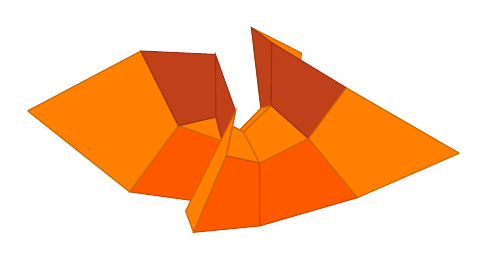
\begin{tikzpicture}
            \begin{axis}[
                view={150}{30},
                samples=\samplescalar, 
                samples y=\samplescalar,
                domain=-1.3:1.3, 
                y domain=-1.3:1.3,
                scale=0.8,
                axis lines=none,
                %colormap/viridis,
                colormap={orangered}{
                            rgb(0cm)=(1,0.2,0);
                            rgb(1cm)=(1,0.5,0);
                            rgb(2cm)=(0.5,0,0.2);
                        },
            ]
            
            % Enneperjeva ploskev 
            \addplot3[
                surf,
                z buffer = sort,
            ]
            (
                {x - (1/3) * x^3 + x * y^2}, 
                {-y - x^2 * y + (1/3) * y^3}, 
                {x^2 - y^2} 
            );

            \end{axis}
        \end{tikzpicture}

        \caption{Enneperjeva ploskev}
    \end{figure}

    Za Gaussovo preslikavo izberemo $\mathfrak{g}(z)=z$. Če vzamemo $\partial X_3=2 z \mathrm{d} z$ dobimo Enneperjevo ploskev, če pa vzamemo $\partial X_3=\frac{\mathrm{d} z}{z}$ pa dobimo katenoid. Eksplicitno povedano: 
    \begin{equation*}
        \text { Enneperjeva ploskev } \quad X(\zeta)=\Re \int_0^\zeta\left(\frac{1}{2}\left(\frac{1}{z}-z\right), \frac{\mathfrak{i}}{2}\left(\frac{1}{z}+z\right), 1\right) 2 z \, \mathrm{d} z,
    \end{equation*}  
    \begin{equation*}
        \text { Katenoida } \quad X(\zeta)=(1,0,0)-\Re \int_1^\zeta\left(\frac{1}{2}\left(\frac{1}{z} - z\right), \frac{\mathfrak{i}}{2}\left(\frac{1}{z}+z\right), 1\right) \frac{\mathrm{d} z}{z} .
    \end{equation*}
\end{frame}

\begin{frame}
    \frametitle{Holomorfne ničelne krivulje}

    Holomorfna imerzija $F=\left(F_1, \ldots, F_n\right): D \rightarrow \mathbb{C}^n$ za $n\geq 3$ in $D\subset \mathbb{C}$, ki zadošča  
    \begin{equation*}
        \left(F_1^{\prime}\right)^2+\left(F_2^{\prime}\right)^2+\cdots+\left(F_n^{\prime}\right)^2=0      
    \end{equation*}
    je \textcolor{red1}{holomorfna ničelna krivulja}. Vsaka taka je oblike 
    \begin{equation*}
        F(z)=c+\int_{z_0}^z f(\zeta) \, \mathrm{d} \zeta, \quad z \in D
    \end{equation*}
    kjer je $c \in \mathbb{C}^n$ in $f:D \rightarrow \mathbb{A}_*$ holomorfna preslikava, za katero velja
    \begin{equation*}
        \oint_C f \, \mathrm{d} z=0 \quad \text { za vsako krivuljo } [C] \in H_1(D, \mathbb{Z}). 
    \end{equation*}
    \begin{posledica}
        Če je $D$ enostavno povezana domena v $\mathbb{C}$, potem vsaka holomorfna preslikava $f: D \rightarrow \mathbb{A}_* \subset \mathbb{C}^n$ določa holomorfno ničelno kirvuljo po formuli $F(z)=c+\int_{z_0}^z f(\zeta) \, \mathrm{d} \zeta$.  
    \end{posledica}
    Če je $F=X+\mathfrak{i} Y: D \rightarrow \mathbb{C}^n$ holomorfna ničelna krivulja, potem sta njen realni del $X=\Re F: D \rightarrow \mathbb{R}^n$ in njen imaginarni del $Y=\Im F: D \rightarrow \mathbb{R}^n$ konformni minimalni ploskvi. Po drugi strani, pa je vsaka konformna minimalna ploskev lokalno (na vsaki enostavni povezani domeni) relani del holomorfne ničelne krivulje. 
    
\end{frame}

\begin{frame}
    \frametitle{Primer: katenoid in helikoid}

    Ker sta $X$ in $Y$ harmonični konjugiranki, pravimo, da sta \textcolor{red1}{konjugirani minimalni ploskvi}. Konformnim minimalnim ploskvam iz 1-parametrične družine 
    \begin{equation*}
        G_t=\Re\left(\mathrm{e}^{\mathfrak{i} t} F\right): D \longrightarrow \mathbb{R}^n, \quad \text{za }t \in \mathbb{R}
    \end{equation*}
    pravimo \textcolor{red1}{pridružene minimalne ploskve} holomorfne ničelne krivulje $Z$.
    
    \vspace{0.8em}

    \textcolor{red1}{Primer:}

    Katenoid in helikoid sta konjugirani minimalni ploskvi - realen in imaginaren del ničelne krivulje 
    \begin{equation*}
        F(\zeta)=(\cos \zeta, \sin \zeta,-i \zeta), \quad \zeta=x+\mathfrak{i} y \in \mathbb{C}        
    \end{equation*}

    Oglejmo si družino minimalnih ploskev glede na relani parameter $(t \in \mathbb{R})$:
    \begin{align*}
        G_t(\zeta) & =\Re\left(e^{i t} F(\zeta)\right) \\
        & =\cos t\begin{pmatrix}
        \cos x \cdot \cosh y \\
        \sin x \cdot \cosh y \\
        y
        \end{pmatrix}+\sin t\begin{pmatrix}
        \sin x \cdot \sinh y \\
        -\cos x \cdot \sinh y \\
        x
        \end{pmatrix}
    \end{align*}
    Pri $t=0$ imamo katenoid in pri $t= \pm \pi / 2$ pa helikoid. 

\end{frame}

\begin{frame}
    \frametitle{Helikatenoid}

    \begin{figure}[ht]
        \centering
        \animategraphics[controls, loop, autoplay, width=0.6\linewidth]{10}{../Slike/animation/73de0b4e-17ea-4815-baa5-68b27a43edf3-}{0}{99}
        \caption{Hleikatenoid animacija}
    \end{figure}
\end{frame}

\begin{frame}
    \begin{center}
        \LARGE \textcolor{red1}{HVALA ZA POZORNOST!}

        \centering
        \begin{figure}
            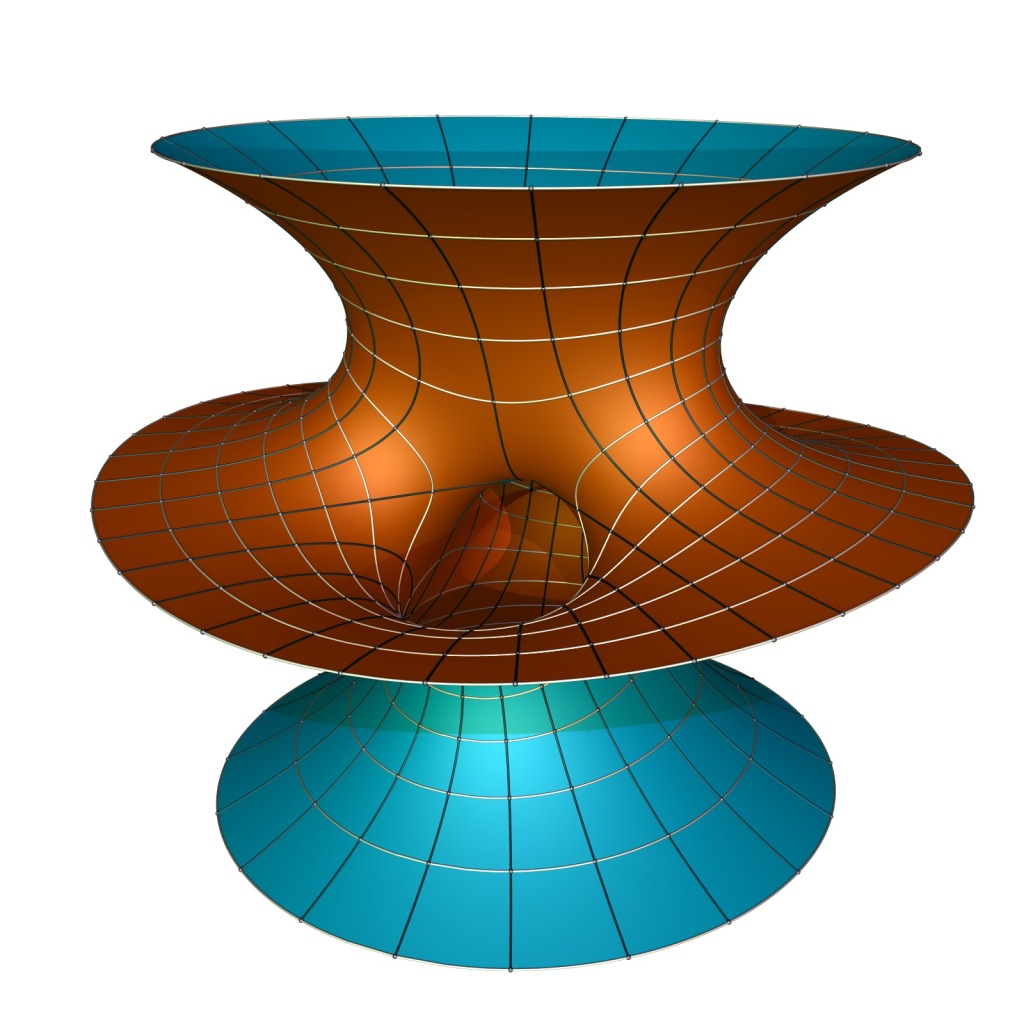
\includegraphics[width=16em]{../Slike/Costa_Minimal_Surface.jpg}
        \end{figure}
    \end{center}

\end{frame}

\end{document}